\begin{longtable}{r l p{5cm} p{3cm}}
	\hline
	\multicolumn{3}{c}{Fonte} & Requisito\tabularnewline
	\midrule
	\midrule
	&  & Capitolato & \hyperlink{R-3V1}{R-3V1}
	
	\hyperlink{R-3V2}{R-3V2}
	
	\hyperlink{R-3V3}{R-3V3}
	
	\hyperlink{R-3V3.1}{R-3V3.1}
	
	\hyperlink{R-3V3.2}{R-3V3.2}
	
	\hyperlink{R-3V4}{R-3V4}
	
	\hyperlink{R-3V3.3}{R-3V3.3}
	
	\hyperlink{R-3V5}{R-3V5}
	
	\hyperlink{R-3V6}{R-3V6}
	
	\hyperlink{R-3V6.1}{R-3V6.1}
	
	\hyperlink{R-3V6.2}{R-3V6.2}
	
	\hyperlink{R-3F7.1}{R-3F7.1}
	
	\hyperlink{R-3F7.5.1}{R-3F7.5.1}
	
	\hyperlink{R-3F7.2}{R-3F7.2}
	
	\hyperlink{R-3F7.3}{R-3F7.3}
	
	\hyperlink{R-2F7.5.2}{R-2F7.5.2}
	
	\hyperlink{R-3F7.4}{R-3F7.4}
	
	\hyperlink{R-3F7.5}{R-3F7.5}
	
	\hyperlink{R-3F7}{R-3F7}
	
	\hyperlink{R-3F7.7}{R-3F7.7}
	
	\hyperlink{R-3F8}{R-3F8}
	
	\hyperlink{R-3V10}{R-3V10}
	
	\hyperlink{R-3V3.4}{R-3V3.4}
	
	\hyperlink{R-2F7.8}{R-2F7.8}
	
	\hyperlink{R-2F7.9}{R-2F7.9}
	
	\hyperlink{R-2F7.10}{R-2F7.10}
	
	\hyperlink{R-2F7.10.1}{R-2F7.10.1}
	
	\hyperlink{R-2F7.10.2}{R-2F7.10.2}
	
	\hyperlink{R-2F7.10.3}{R-2F7.10.3}
	
	\hyperlink{R-3F7.5.5}{R-3F7.5.5}
	
	\hyperlink{R-3F7.5.1.2}{R-3F7.5.1.2}\tabularnewline
	\hline
	&  & Proponente & \hyperlink{R-3F7.5.3}{R-3F7.5.3}
	
	\hyperlink{R-2F7.5.4}{R-2F7.5.4}
	
	\hyperlink{R-2F7.6}{R-2F7.6}\tabularnewline
	\hline
	&  & Committente & \tabularnewline
	\hline
	&  & Interno & \hyperlink{R-3V10}{R-3V10}
	
	\hyperlink{R-3F9.1}{R-3F9.1}
	
	\hyperlink{R-3F18.1}{R-3F18.1}
	
	\hyperlink{R-3Q25}{R-3Q25}
	
	\hyperlink{R-3Q26}{R-3Q26}
	
	\hyperlink{R-3Q27}{R-3Q27}
	
	\hyperlink{R-2Q28}{R-2Q28}\tabularnewline
	\hline
	& \hyperlink{UC1}{UC1} & \hyperlink{UC1}{Autenticazione} & \hyperlink{R-3F31}{R-3F31}\tabularnewline
	\hline
	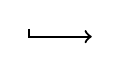
\begin{tikzpicture}
	\draw [->, thick] (0.2,0.2) -- (0.2,0.1) -- (1,0.1);
	\end{tikzpicture} & \hyperlink{UC1.1}{UC1.1} & \hyperlink{UC1.1}{Inserimento username} & \hyperlink{R-3F31.1}{R-3F31.1}\tabularnewline
	\hline
	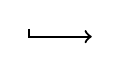
\begin{tikzpicture}
	\draw [->, thick] (0.2,0.2) -- (0.2,0.1) -- (1,0.1);
	\end{tikzpicture} & \hyperlink{UC1.2}{UC1.2} & \hyperlink{UC1.2}{Inserimento password} & \hyperlink{R-3F31.1}{R-3F31.1}\tabularnewline
	\hline
	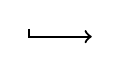
\begin{tikzpicture}
	\draw [->, thick] (0.2,0.2) -- (0.2,0.1) -- (1,0.1);
	\end{tikzpicture} & \hyperlink{UC1.3}{UC1.3} & \hyperlink{UC1.3}{Errore username non presente} & \hyperlink{R-3F31.1.1}{R-3F31.1.1}\tabularnewline
	\hline
	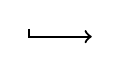
\begin{tikzpicture}
	\draw [->, thick] (0.2,0.2) -- (0.2,0.1) -- (1,0.1);
	\end{tikzpicture} & \hyperlink{UC1.4}{UC1.4} & \hyperlink{UC1.4}{Errore password errata} & \hyperlink{R-3F31.1.2}{R-3F31.1.2}\tabularnewline
	\hline
	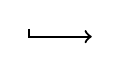
\begin{tikzpicture}
	\draw [->, thick] (0.2,0.2) -- (0.2,0.1) -- (1,0.1);
	\end{tikzpicture} & \hyperlink{UC1.5}{UC1.5} & \hyperlink{UC1.5}{Recupero password} & \hyperlink{R-2F21}{R-2F21}
	
	\hyperlink{R-2F21.1}{R-2F21.1}
	
	\hyperlink{R-2F21.2}{R-2F21.2}\tabularnewline
	\hline
	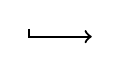
\begin{tikzpicture}
	\draw [->, thick] (0.2,0.2) -- (0.2,0.1) -- (1,0.1);
	\end{tikzpicture} & \hyperlink{UC1.6}{UC1.6} & \hyperlink{UC1.6}{Errore mail per recupero password non presente} & \hyperlink{R-2F21.2}{R-2F21.2}\tabularnewline
	\hline
	& \hyperlink{UC2}{UC2} & \hyperlink{UC2}{Registrazione} & \hyperlink{R-3F9}{R-3F9}\tabularnewline
	\hline
	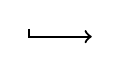
\begin{tikzpicture}
	\draw [->, thick] (0.2,0.2) -- (0.2,0.1) -- (1,0.1);
	\end{tikzpicture} & \hyperlink{UC2.1}{UC2.1} & \hyperlink{UC2.1}{Inserimento nome completo} & \hyperlink{R-3F9.2}{R-3F9.2}
	
	\hyperlink{R-3F9.2.2}{R-3F9.2.2}\tabularnewline
	\hline
	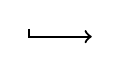
\begin{tikzpicture}
	\draw [->, thick] (0.2,0.2) -- (0.2,0.1) -- (1,0.1);
	\end{tikzpicture} & \hyperlink{UC2.2}{UC2.2} & \hyperlink{UC2.2}{Inserimento username} & \hyperlink{R-3F9.2}{R-3F9.2}\tabularnewline
	\hline
	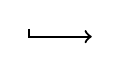
\begin{tikzpicture}
	\draw [->, thick] (0.2,0.2) -- (0.2,0.1) -- (1,0.1);
	\end{tikzpicture} & \hyperlink{UC2.3}{UC2.3} & \hyperlink{UC2.3}{Inserimento password} & \hyperlink{R-3F9.2}{R-3F9.2}\tabularnewline
	\hline
	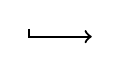
\begin{tikzpicture}
	\draw [->, thick] (0.2,0.2) -- (0.2,0.1) -- (1,0.1);
	\end{tikzpicture} & \hyperlink{UC2.4}{UC2.4} & \hyperlink{UC2.4}{Errore nome completo troppo corto} & \hyperlink{R-3F9.2.1}{R-3F9.2.1}\tabularnewline
	\hline
	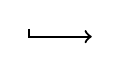
\begin{tikzpicture}
	\draw [->, thick] (0.2,0.2) -- (0.2,0.1) -- (1,0.1);
	\end{tikzpicture} & \hyperlink{UC2.5}{UC2.5} & \hyperlink{UC2.5}{Errore username troppo corto} & \hyperlink{R-3F9.2.1}{R-3F9.2.1}\tabularnewline
	\hline
	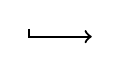
\begin{tikzpicture}
	\draw [->, thick] (0.2,0.2) -- (0.2,0.1) -- (1,0.1);
	\end{tikzpicture} & \hyperlink{UC2.6}{UC2.6} & \hyperlink{UC2.6}{Errore password troppo corta} & \hyperlink{R-3F9.4}{R-3F9.4}
	
	\hyperlink{R-3F9.2.1}{R-3F9.2.1}\tabularnewline
	\hline
	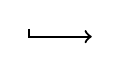
\begin{tikzpicture}
	\draw [->, thick] (0.2,0.2) -- (0.2,0.1) -- (1,0.1);
	\end{tikzpicture} & \hyperlink{UC2.7}{UC2.7} & \hyperlink{UC2.7}{Errore username già utilizzato} & \hyperlink{R-3F9.3}{R-3F9.3}
	
	\hyperlink{R-3F9.5}{R-3F9.5}
	
	\hyperlink{R-3F9.2.1}{R-3F9.2.1}\tabularnewline
	\hline
	& \hyperlink{UC10}{UC10} & \hyperlink{UC10}{Gestione profilo} & \hyperlink{R-3F13}{R-3F13}
	
	\hyperlink{R-3F13.1}{R-3F13.1}
	
	\hyperlink{R-3F13.2}{R-3F13.2}
	
	\hyperlink{R-3F13.1.1}{R-3F13.1.1}
	
	\hyperlink{R-3F13.2.1}{R-3F13.2.1}
	
	\hyperlink{R-3F13.3}{R-3F13.3}
	
	\hyperlink{R-3F13.3.1}{R-3F13.3.1}
	
	\hyperlink{R-3F13.3.2}{R-3F13.3.2}
	
	\hyperlink{R-3F13.2.1.1}{R-3F13.2.1.1}
	
	\hyperlink{R-3F13.2.2}{R-3F13.2.2}
	
	\hyperlink{R-3F13.2.2.1}{R-3F13.2.2.1}
	
	\hyperlink{R-3F13.3.3}{R-3F13.3.3}
	
	\hyperlink{R-3F13.1.2}{R-3F13.1.2}
	
	\hyperlink{R-3F13.3.4}{R-3F13.3.4}\tabularnewline
	\hline
	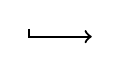
\begin{tikzpicture}
	\draw [->, thick] (0.2,0.2) -- (0.2,0.1) -- (1,0.1);
	\end{tikzpicture} & \hyperlink{UC10.1}{UC10.1} & \hyperlink{UC10.1}{Modifica nome completo} & \hyperlink{R-3F13.3}{R-3F13.3}
	
	\hyperlink{R-3F13.3.1}{R-3F13.3.1}
	
	\hyperlink{R-3F13.3.3}{R-3F13.3.3}\tabularnewline
	\hline
	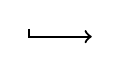
\begin{tikzpicture}
	\draw [->, thick] (0.2,0.2) -- (0.2,0.1) -- (1,0.1);
	\end{tikzpicture} & \hyperlink{UC10.2}{UC10.2} & \hyperlink{UC10.2}{Modifica username} & \hyperlink{R-3F13.1}{R-3F13.1}
	
	\hyperlink{R-3F13.1.1}{R-3F13.1.1}
	
	\hyperlink{R-3F13.3}{R-3F13.3}
	
	\hyperlink{R-3F13.3.2}{R-3F13.3.2}
	
	\hyperlink{R-3F13.3.4}{R-3F13.3.4}\tabularnewline
	\hline
	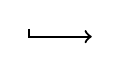
\begin{tikzpicture}
	\draw [->, thick] (0.2,0.2) -- (0.2,0.1) -- (1,0.1);
	\end{tikzpicture} & \hyperlink{UC10.3}{UC10.3} & \hyperlink{UC10.3}{Modifica password} & \hyperlink{R-3F13.2}{R-3F13.2}
	
	\hyperlink{R-3F13.2.1}{R-3F13.2.1}
	
	\hyperlink{R-3F13.2.2}{R-3F13.2.2}
	
	\hyperlink{R-3F13.2.2.1}{R-3F13.2.2.1}\tabularnewline
	\hline
	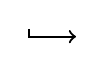
\begin{tikzpicture}
	\draw [->, thick] (0.4,0.2) -- (0.4,0.1) -- (1,0.1);
	\end{tikzpicture} & \hyperlink{UC10.3.1}{UC10.3.1} & \hyperlink{UC10.3.1}{Inserimento vecchia password} & \hyperlink{R-3F13.2.1}{R-3F13.2.1}\tabularnewline
	\hline
	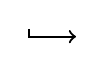
\begin{tikzpicture}
	\draw [->, thick] (0.4,0.2) -- (0.4,0.1) -- (1,0.1);
	\end{tikzpicture} & \hyperlink{UC10.3.2}{UC10.3.2} & \hyperlink{UC10.3.2}{Errore password non corrispondente} & \hyperlink{R-3F13.2.1.1}{R-3F13.2.1.1}\tabularnewline
	\hline
	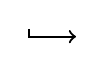
\begin{tikzpicture}
	\draw [->, thick] (0.4,0.2) -- (0.4,0.1) -- (1,0.1);
	\end{tikzpicture} & \hyperlink{UC10.3.3}{UC10.3.3} & \hyperlink{UC10.3.3}{Inserimento nuova password} & \hyperlink{R-3F13.2}{R-3F13.2}\tabularnewline
	\hline
	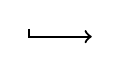
\begin{tikzpicture}
	\draw [->, thick] (0.2,0.2) -- (0.2,0.1) -- (1,0.1);
	\end{tikzpicture} & \hyperlink{UC10.4}{UC10.4} & \hyperlink{UC10.4}{Errore username troppo corto} & \hyperlink{R-3F13.1.1}{R-3F13.1.1}
	
	\hyperlink{R-3F13.3.4}{R-3F13.3.4}\tabularnewline
	\hline
	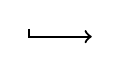
\begin{tikzpicture}
	\draw [->, thick] (0.2,0.2) -- (0.2,0.1) -- (1,0.1);
	\end{tikzpicture} & \hyperlink{UC10.5}{UC10.5} & \hyperlink{UC10.5}{Errore nome completo troppo corto} & \hyperlink{R-3F13.3.3}{R-3F13.3.3}\tabularnewline
	\hline
	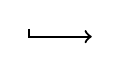
\begin{tikzpicture}
	\draw [->, thick] (0.2,0.2) -- (0.2,0.1) -- (1,0.1);
	\end{tikzpicture} & \hyperlink{UC10.6}{UC10.6} & \hyperlink{UC10.6}{Errore username già utilizzato} & \hyperlink{R-3F13.1.1}{R-3F13.1.1}
	
	\hyperlink{R-3F13.1.2}{R-3F13.1.2}\tabularnewline
	\hline
	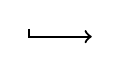
\begin{tikzpicture}
	\draw [->, thick] (0.2,0.2) -- (0.2,0.1) -- (1,0.1);
	\end{tikzpicture} & \hyperlink{UC10.7}{UC10.7} & \hyperlink{UC10.7}{Errore password troppo corta} & \hyperlink{R-3F13.2.1.1}{R-3F13.2.1.1}
	
	\hyperlink{R-3F13.2.2.1}{R-3F13.2.2.1}\tabularnewline
	\hline
	& \hyperlink{UC11}{UC11} & \hyperlink{UC11}{Logout} & \hyperlink{R-3F17}{R-3F17}\tabularnewline
	\hline
	& \hyperlink{UC17}{UC17} & \hyperlink{UC17}{Gestione domande} & \hyperlink{R-3F7.2}{R-3F7.2}
	
	\hyperlink{R-3F7.11}{R-3F7.11}
	
	\hyperlink{R-3F7.11.1}{R-3F7.11.1}
	
	\hyperlink{R-3F7.11.2}{R-3F7.11.2}
	
	\hyperlink{R-3F7.11.3}{R-3F7.11.3}
	
	\hyperlink{R-3F7.11.1.1}{R-3F7.11.1.1}
	
	\hyperlink{R-3F7.11.1.2}{R-3F7.11.1.2}
	
	\hyperlink{R-3F7.11.1.1.1}{R-3F7.11.1.1.1}
	
	\hyperlink{R-3F7.11.1.2.1}{R-3F7.11.1.2.1}\tabularnewline
	\hline
	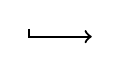
\begin{tikzpicture}
	\draw [->, thick] (0.2,0.2) -- (0.2,0.1) -- (1,0.1);
	\end{tikzpicture} & \hyperlink{UC17.1}{UC17.1} & \hyperlink{UC17.1}{Inserimento domanda} & \hyperlink{R-2F7.5.2}{R-2F7.5.2}
	
	\hyperlink{R-3F7.5.3}{R-3F7.5.3}
	
	\hyperlink{R-3F7.11.1}{R-3F7.11.1}
	
	\hyperlink{R-3F7.11.1.1}{R-3F7.11.1.1}
	
	\hyperlink{R-3F7.11.1.2.2}{R-3F7.11.1.2.2}
	
	\hyperlink{R-3F7.11.1.2.3}{R-3F7.11.1.2.3}
	
	\hyperlink{R-1F7.11.1.2.4}{R-1F7.11.1.2.4}
	
	\hyperlink{R-1F7.11.1.2.5}{R-1F7.11.1.2.5}
	
	\hyperlink{R-1F7.11.1.2.6}{R-1F7.11.1.2.6}
	
	\hyperlink{R-2F7.11.1.2.7}{R-2F7.11.1.2.7}
	
	\hyperlink{R-3F7.5.5}{R-3F7.5.5}
	
	\hyperlink{R-1F7.11.1.2.8}{R-1F7.11.1.2.8}
	
	\hyperlink{R-1F7.11.1.2.9}{R-1F7.11.1.2.9}\tabularnewline
	\hline
	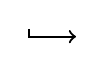
\begin{tikzpicture}
	\draw [->, thick] (0.4,0.2) -- (0.4,0.1) -- (1,0.1);
	\end{tikzpicture} & \hyperlink{UC17.1.1}{UC17.1.1} & \hyperlink{UC17.1.1}{Selezione argomenti nuova domanda} & \hyperlink{R-3F7.11.1.1}{R-3F7.11.1.1}
	
	\hyperlink{R-3F7.11.1.1.1}{R-3F7.11.1.1.1}\tabularnewline
	\hline
	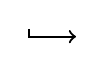
\begin{tikzpicture}
	\draw [->, thick] (0.4,0.2) -- (0.4,0.1) -- (1,0.1);
	\end{tikzpicture} & \hyperlink{UC17.1.2}{UC17.1.2} & \hyperlink{UC17.1.2}{Scrittura nuova domanda in QML} & \hyperlink{R-3F7.5.1}{R-3F7.5.1}
	
	\hyperlink{R-3F7.5}{R-3F7.5}
	
	\hyperlink{R-3F7.11.1.2}{R-3F7.11.1.2}
	
	\hyperlink{R-3F7.11.1.2.1}{R-3F7.11.1.2.1}
	
	\hyperlink{R-2F7.5.1.1}{R-2F7.5.1.1}
	
	\hyperlink{R-3F7.5.1.2}{R-3F7.5.1.2}
	
	\hyperlink{R-2F7.5.1.3}{R-2F7.5.1.3}
	
	\hyperlink{R-2F7.5.1.4}{R-2F7.5.1.4}
	
	\hyperlink{R-2F7.5.1.5}{R-2F7.5.1.5}
	
	\hyperlink{R-3F7.5.1.6}{R-3F7.5.1.6}
	
	\hyperlink{R-2F7.5.1.7}{R-2F7.5.1.7}
	
	\hyperlink{R-2F7.5.1.8}{R-2F7.5.1.8}
	
	\hyperlink{R-1F7.16}{R-1F7.16}\tabularnewline
	\hline
	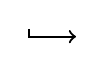
\begin{tikzpicture}
	\draw [->, thick] (0.4,0.2) -- (0.4,0.1) -- (1,0.1);
	\end{tikzpicture} & \hyperlink{UC17.1.3}{UC17.1.3} & \hyperlink{UC17.1.3}{Errore QML non valido} & \hyperlink{R-3F7.11.1.2.1}{R-3F7.11.1.2.1}\tabularnewline
	\hline
	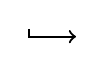
\begin{tikzpicture}
	\draw [->, thick] (0.4,0.2) -- (0.4,0.1) -- (1,0.1);
	\end{tikzpicture} & \hyperlink{UC17.1.4}{UC17.1.4} & \hyperlink{UC17.1.4}{Errore argomento mancante} & \hyperlink{R-3F7.11.1.1.1}{R-3F7.11.1.1.1}\tabularnewline
	\hline
	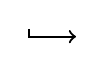
\begin{tikzpicture}
	\draw [->, thick] (0.4,0.2) -- (0.4,0.1) -- (1,0.1);
	\end{tikzpicture} & \hyperlink{UC17.1.5}{UC17.1.5} & \hyperlink{UC17.1.5}{Scrittura nuova domanda da interfaccia grafica} & \hyperlink{R-2F7.5.4}{R-2F7.5.4}
	
	\hyperlink{R-2F7.5.1.7}{R-2F7.5.1.7}
	
	\hyperlink{R-2F7.5.1.8}{R-2F7.5.1.8}\tabularnewline
	\hline
	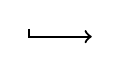
\begin{tikzpicture}
	\draw [->, thick] (0.2,0.2) -- (0.2,0.1) -- (1,0.1);
	\end{tikzpicture} & \hyperlink{UC17.2}{UC17.2} & \hyperlink{UC17.2}{Modifica domanda} & \hyperlink{R-3F7.11.2}{R-3F7.11.2}\tabularnewline
	\hline
	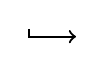
\begin{tikzpicture}
	\draw [->, thick] (0.4,0.2) -- (0.4,0.1) -- (1,0.1);
	\end{tikzpicture} & \hyperlink{UC17.2.1}{UC17.2.1} & \hyperlink{UC17.2.1}{Selezione argomenti modifica domanda} & \hyperlink{R-3F7.11.2}{R-3F7.11.2}\tabularnewline
	\hline
	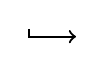
\begin{tikzpicture}
	\draw [->, thick] (0.4,0.2) -- (0.4,0.1) -- (1,0.1);
	\end{tikzpicture} & \hyperlink{UC17.2.2}{UC17.2.2} & \hyperlink{UC17.2.2}{Scrittura domanda in QML della domanda da modificare} & \hyperlink{R-3F7.11.2}{R-3F7.11.2}\tabularnewline
	\hline
	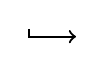
\begin{tikzpicture}
	\draw [->, thick] (0.4,0.2) -- (0.4,0.1) -- (1,0.1);
	\end{tikzpicture} & \hyperlink{UC17.2.3}{UC17.2.3} & \hyperlink{UC17.2.3}{Modifica domanda da interfaccia grafica} & \hyperlink{R-3F7.11.2}{R-3F7.11.2}\tabularnewline
	\hline
	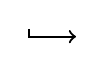
\begin{tikzpicture}
	\draw [->, thick] (0.4,0.2) -- (0.4,0.1) -- (1,0.1);
	\end{tikzpicture} & \hyperlink{UC17.2.4}{UC17.2.4} & \hyperlink{UC17.2.4}{Errore modifica QML non valido} & \hyperlink{R-3F7.11.1.2.1}{R-3F7.11.1.2.1}\tabularnewline
	\hline
	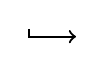
\begin{tikzpicture}
	\draw [->, thick] (0.4,0.2) -- (0.4,0.1) -- (1,0.1);
	\end{tikzpicture} & \hyperlink{UC17.2.5}{UC17.2.5} & \hyperlink{UC17.2.5}{Errore argomento mancante} & \hyperlink{R-3F7.11.1.1.2}{R-3F7.11.1.1.2}\tabularnewline
	\hline
	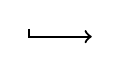
\begin{tikzpicture}
	\draw [->, thick] (0.2,0.2) -- (0.2,0.1) -- (1,0.1);
	\end{tikzpicture} & \hyperlink{UC17.3}{UC17.3} & \hyperlink{UC17.3}{Elimina domanda} & \hyperlink{R-3F7.11.3}{R-3F7.11.3}\tabularnewline
	\hline
	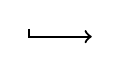
\begin{tikzpicture}
	\draw [->, thick] (0.2,0.2) -- (0.2,0.1) -- (1,0.1);
	\end{tikzpicture} & \hyperlink{UC17.4}{UC17.4} & \hyperlink{UC17.4}{Inserimento domanda di tipo vero/falso} & \hyperlink{R-3F7.11.1.2.2}{R-3F7.11.1.2.2}
	
	\hyperlink{R-3F7.5.5}{R-3F7.5.5}\tabularnewline
	\hline
	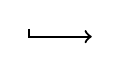
\begin{tikzpicture}
	\draw [->, thick] (0.2,0.2) -- (0.2,0.1) -- (1,0.1);
	\end{tikzpicture} & \hyperlink{UC17.5}{UC17.5} & \hyperlink{UC17.5}{Inserimento domanda a scelta multipla} & \hyperlink{R-2F7.5.2}{R-2F7.5.2}
	
	\hyperlink{R-3F7.11.1.2.3}{R-3F7.11.1.2.3}\tabularnewline
	\hline
	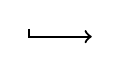
\begin{tikzpicture}
	\draw [->, thick] (0.2,0.2) -- (0.2,0.1) -- (1,0.1);
	\end{tikzpicture} & \hyperlink{UC17.6}{UC17.6} & \hyperlink{UC17.6}{Inserimento domanda a risposta multipla} & \hyperlink{R-1F7.11.1.2.4}{R-1F7.11.1.2.4}
	
	\hyperlink{R-3F7.5.5}{R-3F7.5.5}\tabularnewline
	\hline
	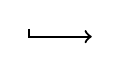
\begin{tikzpicture}
	\draw [->, thick] (0.2,0.2) -- (0.2,0.1) -- (1,0.1);
	\end{tikzpicture} & \hyperlink{UC17.7}{UC17.7} & \hyperlink{UC17.7}{Inserimento domanda di tipo testo con parole omesse} & \hyperlink{R-2F7.5.2}{R-2F7.5.2}
	
	\hyperlink{R-1F7.11.1.2.5}{R-1F7.11.1.2.5}\tabularnewline
	\hline
	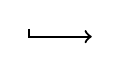
\begin{tikzpicture}
	\draw [->, thick] (0.2,0.2) -- (0.2,0.1) -- (1,0.1);
	\end{tikzpicture} & \hyperlink{UC17.8}{UC17.8} & \hyperlink{UC17.8}{Inserimento domanda con l'associazione di parole} & \hyperlink{R-2F7.5.2}{R-2F7.5.2}
	
	\hyperlink{R-1F7.11.1.2.6}{R-1F7.11.1.2.6}\tabularnewline
	\hline
	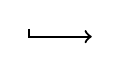
\begin{tikzpicture}
	\draw [->, thick] (0.2,0.2) -- (0.2,0.1) -- (1,0.1);
	\end{tikzpicture} & \hyperlink{UC17.9}{UC17.9} & \hyperlink{UC17.9}{Inserimento domanda a risposta aperta} & \hyperlink{R-2F7.5.2}{R-2F7.5.2}
	
	\hyperlink{R-2F7.11.1.2.7}{R-2F7.11.1.2.7}\tabularnewline
	\hline
	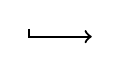
\begin{tikzpicture}
	\draw [->, thick] (0.2,0.2) -- (0.2,0.1) -- (1,0.1);
	\end{tikzpicture} & \hyperlink{UC17.10}{UC17.10} & \hyperlink{UC17.10}{Visualizza domanda} & \hyperlink{R-3F7.2}{R-3F7.2}
	
	\hyperlink{R-3F29}{R-3F29}\tabularnewline
	\hline
	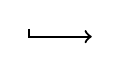
\begin{tikzpicture}
	\draw [->, thick] (0.2,0.2) -- (0.2,0.1) -- (1,0.1);
	\end{tikzpicture} & \hyperlink{UC17.11}{UC17.11} & \hyperlink{UC17.11}{Errore eliminazione domanda utilizzata} & \hyperlink{R-3F7.11.3.1}{R-3F7.11.3.1}\tabularnewline
	\hline
	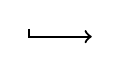
\begin{tikzpicture}
	\draw [->, thick] (0.2,0.2) -- (0.2,0.1) -- (1,0.1);
	\end{tikzpicture} & \hyperlink{UC17.12}{UC17.12} & \hyperlink{UC17.12}{Inserimento domanda ad ordinamento} & \hyperlink{R-1F7.11.1.2.8}{R-1F7.11.1.2.8}\tabularnewline
	\hline
	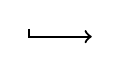
\begin{tikzpicture}
	\draw [->, thick] (0.2,0.2) -- (0.2,0.1) -- (1,0.1);
	\end{tikzpicture} & \hyperlink{UC17.13}{UC17.13} & \hyperlink{UC17.13}{Inserimento domanda a tolleranza numerica } & \hyperlink{R-1F7.11.1.2.9}{R-1F7.11.1.2.9}\tabularnewline
	\hline
	& \hyperlink{UC18}{UC18} & \hyperlink{UC18}{Gestione questionari} & \hyperlink{R-3F7.2}{R-3F7.2}
	
	\hyperlink{R-3F7.3}{R-3F7.3}
	
	\hyperlink{R-3F7}{R-3F7}
	
	\hyperlink{R-3F7.7}{R-3F7.7}
	
	\hyperlink{R-3F7.11}{R-3F7.11}
	
	\hyperlink{R-3F7.12}{R-3F7.12}
	
	\hyperlink{R-3F7.12.2}{R-3F7.12.2}
	
	\hyperlink{R-3F7.12.3}{R-3F7.12.3}
	
	\hyperlink{R-3F7.13}{R-3F7.13}
	
	\hyperlink{R-3F7.12.4}{R-3F7.12.4}
	
	\hyperlink{R-3F7.7.1}{R-3F7.7.1}\tabularnewline
	\hline
	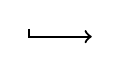
\begin{tikzpicture}
	\draw [->, thick] (0.2,0.2) -- (0.2,0.1) -- (1,0.1);
	\end{tikzpicture} & \hyperlink{UC18.1}{UC18.1} & \hyperlink{UC18.1}{Inserisci questionario} & \hyperlink{R-3F7.7}{R-3F7.7}
	
	\hyperlink{R-3F7.7.1}{R-3F7.7.1}
	
	\hyperlink{R-3F7.14}{R-3F7.14}\tabularnewline
	\hline
	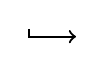
\begin{tikzpicture}
	\draw [->, thick] (0.4,0.2) -- (0.4,0.1) -- (1,0.1);
	\end{tikzpicture} & \hyperlink{UC18.1.1}{UC18.1.1} & \hyperlink{UC18.1.1}{Aggiungi domanda in un nuovo questionario } & \hyperlink{R-3F7.11}{R-3F7.11}
	
	\hyperlink{R-3F7.11.1.2}{R-3F7.11.1.2}
	
	\hyperlink{R-3F7.11.1.1.1}{R-3F7.11.1.1.1}
	
	\hyperlink{R-3F7.11.1.2.1}{R-3F7.11.1.2.1}\tabularnewline
	\hline
	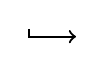
\begin{tikzpicture}
	\draw [->, thick] (0.4,0.2) -- (0.4,0.1) -- (1,0.1);
	\end{tikzpicture} & \hyperlink{UC18.1.2}{UC18.1.2} & \hyperlink{UC18.1.2}{Elimina domanda da un nuovo questionario} & \hyperlink{R-3F7.11}{R-3F7.11}\tabularnewline
	\hline
	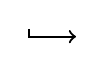
\begin{tikzpicture}
	\draw [->, thick] (0.4,0.2) -- (0.4,0.1) -- (1,0.1);
	\end{tikzpicture} & \hyperlink{UC18.1.3}{UC18.1.3} & \hyperlink{UC18.1.3}{Seleziona argomenti del nuovo questionario} & \hyperlink{R-3F7.14.1}{R-3F7.14.1}\tabularnewline
	\hline
	\begin{tikzpicture}
	\draw [->, thick] (0.2,0.2) -- (0.2,0.1) -- (1,0.1);
	\end{tikzpicture} & \hyperlink{UC18.2}{UC18.2} & \hyperlink{UC18.2}{Modifica questionario} & \hyperlink{R-3F7.12}{R-3F7.12}
	
	\hyperlink{R-3F7.12.4}{R-3F7.12.4}\tabularnewline
	\hline
	\begin{tikzpicture}
	\draw [->, thick] (0.4,0.2) -- (0.4,0.1) -- (1,0.1);
	\end{tikzpicture} & \hyperlink{UC18.2.1}{UC18.2.1} & \hyperlink{UC18.2.1}{Aggiungi domanda in un questionario} & \hyperlink{R-3F7.12.2}{R-3F7.12.2}\tabularnewline
	\hline
	\begin{tikzpicture}
	\draw [->, thick] (0.4,0.2) -- (0.4,0.1) -- (1,0.1);
	\end{tikzpicture} & \hyperlink{UC18.2.2}{UC18.2.2} & \hyperlink{UC18.2.2}{Elimina domanda da un questionario da  modificare} & \hyperlink{R-3F7.12.3}{R-3F7.12.3}\tabularnewline
	\hline
	\begin{tikzpicture}
	\draw [->, thick] (0.4,0.2) -- (0.4,0.1) -- (1,0.1);
	\end{tikzpicture} & \hyperlink{UC18.2.3}{UC18.2.3} & \hyperlink{UC18.2.3}{Selezione argomenti modifica questionario} & \hyperlink{R-3F7.12.4}{R-3F7.12.4}\tabularnewline
	\hline
	\begin{tikzpicture}
	\draw [->, thick] (0.2,0.2) -- (0.2,0.1) -- (1,0.1);
	\end{tikzpicture} & \hyperlink{UC18.3}{UC18.3} & \hyperlink{UC18.3}{Elimina questionario} & \hyperlink{R-3F7.13}{R-3F7.13}\tabularnewline
	\hline
	\begin{tikzpicture}
	\draw [->, thick] (0.2,0.2) -- (0.2,0.1) -- (1,0.1);
	\end{tikzpicture} & \hyperlink{UC18.4}{UC18.4} & \hyperlink{UC18.4}{Errore questionario vuoto} & \hyperlink{R-3F7.7.1}{R-3F7.7.1}\tabularnewline
	\hline
	\begin{tikzpicture}
	\draw [->, thick] (0.2,0.2) -- (0.2,0.1) -- (1,0.1);
	\end{tikzpicture} & \hyperlink{UC18.5}{UC18.5} & \hyperlink{UC18.5}{Visualizza questionario} & \hyperlink{R-3F30}{R-3F30}\tabularnewline
	\hline
	& \hyperlink{UC19}{UC19} & \hyperlink{UC19}{Gestione classi} & \hyperlink{R-2F12.1.1}{R-2F12.1.1}
	
	\hyperlink{R-2F12}{R-2F12}
	
	\hyperlink{R-2F12.1}{R-2F12.1}
	
	\hyperlink{R-2F12.2}{R-2F12.2}
	
	\hyperlink{R-2F12.3}{R-2F12.3}
	
	\hyperlink{R-2F12.1.2}{R-2F12.1.2}
	
	\hyperlink{R-2F12.1.3}{R-2F12.1.3}
	
	\hyperlink{R-2F12.3.1}{R-2F12.3.1}
	
	\hyperlink{R-2F12.3.2}{R-2F12.3.2}
	
	\hyperlink{R-2F12.3.3}{R-2F12.3.3}
	
	\hyperlink{R-2F12.1.1.1}{R-2F12.1.1.1}\tabularnewline
	\hline
	\begin{tikzpicture}
	\draw [->, thick] (0.2,0.2) -- (0.2,0.1) -- (1,0.1);
	\end{tikzpicture} & \hyperlink{UC19.1}{UC19.1} & \hyperlink{UC19.1}{Inserisci classe} & \hyperlink{R-2F7.6}{R-2F7.6}
	
	\hyperlink{R-2F12.1.1}{R-2F12.1.1}
	
	\hyperlink{R-2F12.1}{R-2F12.1}
	
	\hyperlink{R-2F12.1.2}{R-2F12.1.2}
	
	\hyperlink{R-2F12.1.3}{R-2F12.1.3}
	
	\hyperlink{R-2F12.1.1.1}{R-2F12.1.1.1}\tabularnewline
	\hline
	\begin{tikzpicture}
	\draw [->, thick] (0.4,0.2) -- (0.4,0.1) -- (1,0.1);
	\end{tikzpicture} & \hyperlink{UC19.1.1}{UC19.1.1} & \hyperlink{UC19.1.1}{Inserisci nome classe} & \hyperlink{R-2F12.1.1}{R-2F12.1.1}
	
	\hyperlink{R-2F12.3.1}{R-2F12.3.1}
	
	\hyperlink{R-2F12.1.1.1}{R-2F12.1.1.1}\tabularnewline
	\hline
	\begin{tikzpicture}
	\draw [->, thick] (0.4,0.2) -- (0.4,0.1) -- (1,0.1);
	\end{tikzpicture} & \hyperlink{UC19.1.2}{UC19.1.2} & \hyperlink{UC19.1.2}{Inserisci argomenti classe} & \hyperlink{R-2F12.1.2}{R-2F12.1.2}
	
	\hyperlink{R-2F12.3.2}{R-2F12.3.2}\tabularnewline
	\hline
	\begin{tikzpicture}
	\draw [->, thick] (0.4,0.2) -- (0.4,0.1) -- (1,0.1);
	\end{tikzpicture} & \hyperlink{UC19.1.3}{UC19.1.3} & \hyperlink{UC19.1.3}{Inserisci password classe} & \hyperlink{R-2F12.1.3}{R-2F12.1.3}
	
	\hyperlink{R-2F12.3.3}{R-2F12.3.3}\tabularnewline
	\hline
	\begin{tikzpicture}
	\draw [->, thick] (0.2,0.2) -- (0.2,0.1) -- (1,0.1);
	\end{tikzpicture} & \hyperlink{UC19.2}{UC19.2} & \hyperlink{UC19.2}{Modifica classe} & \hyperlink{R-2F12.3}{R-2F12.3}
	
	\hyperlink{R-2F12.3.1}{R-2F12.3.1}
	
	\hyperlink{R-2F12.3.2}{R-2F12.3.2}
	
	\hyperlink{R-2F12.3.3}{R-2F12.3.3}\tabularnewline
	\hline
	\begin{tikzpicture}
	\draw [->, thick] (0.2,0.2) -- (0.2,0.1) -- (1,0.1);
	\end{tikzpicture} & \hyperlink{UC19.3}{UC19.3} & \hyperlink{UC19.3}{Elimina classe} & \hyperlink{R-2F12.2}{R-2F12.2}\tabularnewline
	\hline
	\begin{tikzpicture}
	\draw [->, thick] (0.2,0.2) -- (0.2,0.1) -- (1,0.1);
	\end{tikzpicture} & \hyperlink{UC19.4}{UC19.4} & \hyperlink{UC19.4}{Errore nome classe già presente} & \hyperlink{R-2F12.1.1.1}{R-2F12.1.1.1}\tabularnewline
	\hline
	& \hyperlink{UC20}{UC20} & \hyperlink{UC20}{Gestione argomenti} & \hyperlink{R-3F22}{R-3F22}
	
	\hyperlink{R-3F22.1}{R-3F22.1}
	
	\hyperlink{R-3F22.2}{R-3F22.2}
	
	\hyperlink{R-3F22.3}{R-3F22.3}
	
	\hyperlink{R-3F22.4}{R-3F22.4}
	
	\hyperlink{R-3F22.1.1}{R-3F22.1.1}
	
	\hyperlink{R-3F22.2.1}{R-3F22.2.1}
	
	\hyperlink{R-3F22.2.2}{R-3F22.2.2}\tabularnewline
	\hline
	\begin{tikzpicture}
	\draw [->, thick] (0.2,0.2) -- (0.2,0.1) -- (1,0.1);
	\end{tikzpicture} & \hyperlink{UC20.1}{UC20.1} & \hyperlink{UC20.1}{Crea argomento} & \hyperlink{R-3F22.1}{R-3F22.1}
	
	\hyperlink{R-3F22.1.1}{R-3F22.1.1}\tabularnewline
	\hline
	\begin{tikzpicture}
	\draw [->, thick] (0.2,0.2) -- (0.2,0.1) -- (1,0.1);
	\end{tikzpicture} & \hyperlink{UC20.2}{UC20.2} & \hyperlink{UC20.2}{Errore argomento già presente nel sistema} & \hyperlink{R-3F22.1.1}{R-3F22.1.1}\tabularnewline
	\hline
	\begin{tikzpicture}
	\draw [->, thick] (0.2,0.2) -- (0.2,0.1) -- (1,0.1);
	\end{tikzpicture} & \hyperlink{UC20.3}{UC20.3} & \hyperlink{UC20.3}{Modifica argomento} & \hyperlink{R-3F22.3}{R-3F22.3}\tabularnewline
	\hline
	\begin{tikzpicture}
	\draw [->, thick] (0.2,0.2) -- (0.2,0.1) -- (1,0.1);
	\end{tikzpicture} & \hyperlink{UC20.4}{UC20.4} & \hyperlink{UC20.4}{Eliminazione argomento} & \hyperlink{R-3F22.2}{R-3F22.2}
	
	\hyperlink{R-3F22.2.1}{R-3F22.2.1}
	
	\hyperlink{R-3F22.2.2}{R-3F22.2.2}\tabularnewline
	\hline
	\begin{tikzpicture}
	\draw [->, thick] (0.2,0.2) -- (0.2,0.1) -- (1,0.1);
	\end{tikzpicture} & \hyperlink{UC20.5}{UC20.5} & \hyperlink{UC20.5}{Errore l'argomento ha domande o questionari} & \hyperlink{R-3F22.2.2}{R-3F22.2.2}\tabularnewline
	\hline
	& \hyperlink{UC21}{UC21} & \hyperlink{UC21}{Visualizza statistiche} & \hyperlink{R-2F23.3.1}{R-2F23.3.1}
	
	\hyperlink{R-2F23}{R-2F23}
	
	\hyperlink{R-2F23.1}{R-2F23.1}
	
	\hyperlink{R-2F23.2}{R-2F23.2}
	
	\hyperlink{R-2F23.3}{R-2F23.3}
	
	\hyperlink{R-2F23.1.1}{R-2F23.1.1}
	
	\hyperlink{R-2F23.2.1}{R-2F23.2.1}
	
	\hyperlink{R-2F23.3.2}{R-2F23.3.2}
	
	\hyperlink{R-2F23.3.3}{R-2F23.3.3}
	
	\hyperlink{R-2F23.3.4}{R-2F23.3.4}
	
	\hyperlink{R-2F23.3.4.1}{R-2F23.3.4.1}
	
	\hyperlink{R-2F23.3.5}{R-2F23.3.5}
	
	\hyperlink{R-2F23.3.5.1}{R-2F23.3.5.1}\tabularnewline
	\hline
	& \hyperlink{UC22}{UC22} & \hyperlink{UC22}{Visualizza statistiche domanda} & \hyperlink{R-2F23.1}{R-2F23.1}
	
	\hyperlink{R-2F23.1.1}{R-2F23.1.1}\tabularnewline
	\hline
	& \hyperlink{UC23}{UC23} & \hyperlink{UC23}{Visualizza statistiche questionario} & \hyperlink{R-2F23.2}{R-2F23.2}
	
	\hyperlink{R-2F23.2.1}{R-2F23.2.1}\tabularnewline
	\hline
	& \hyperlink{UC24}{UC24} & \hyperlink{UC24}{Visualizza statistiche classe} & \hyperlink{R-2F23.3.1}{R-2F23.3.1}
	
	\hyperlink{R-2F23.3}{R-2F23.3}
	
	\hyperlink{R-2F23.3.2}{R-2F23.3.2}
	
	\hyperlink{R-2F23.3.3}{R-2F23.3.3}
	
	\hyperlink{R-2F23.3.4}{R-2F23.3.4}
	
	\hyperlink{R-2F23.3.4.1}{R-2F23.3.4.1}
	
	\hyperlink{R-2F23.3.5}{R-2F23.3.5}
	
	\hyperlink{R-2F23.3.5.1}{R-2F23.3.5.1}\tabularnewline
	\hline
	\begin{tikzpicture}
	\draw [->, thick] (0.2,0.2) -- (0.2,0.1) -- (1,0.1);
	\end{tikzpicture} & \hyperlink{UC24.1}{UC24.1} & \hyperlink{UC24.1}{Visualizza risultati domande della classe} & \hyperlink{R-2F23.3.5}{R-2F23.3.5}
	
	\hyperlink{R-2F23.3.5.1}{R-2F23.3.5.1}\tabularnewline
	\hline
	\begin{tikzpicture}
	\draw [->, thick] (0.2,0.2) -- (0.2,0.1) -- (1,0.1);
	\end{tikzpicture} & \hyperlink{UC24.2}{UC24.2} & \hyperlink{UC24.2}{Visualizza risultati questionari della classe} & \hyperlink{R-2F23.3.1}{R-2F23.3.1}\tabularnewline
	\hline
	\begin{tikzpicture}
	\draw [->, thick] (0.2,0.2) -- (0.2,0.1) -- (1,0.1);
	\end{tikzpicture} & \hyperlink{UC24.3}{UC24.3} & \hyperlink{UC24.3}{Visualizza sommario statistiche classe} & \hyperlink{R-2F23.3.3}{R-2F23.3.3}\tabularnewline
	\hline
	\begin{tikzpicture}
	\draw [->, thick] (0.2,0.2) -- (0.2,0.1) -- (1,0.1);
	\end{tikzpicture} & \hyperlink{UC24.4}{UC24.4} & \hyperlink{UC24.4}{Visualizza statistiche studente della classe} & \hyperlink{R-2F23.3.4}{R-2F23.3.4}
	
	\hyperlink{R-2F23.3.4.1}{R-2F23.3.4.1}\tabularnewline
	\hline
	\begin{tikzpicture}
	\draw [->, thick] (0.4,0.2) -- (0.4,0.1) -- (1,0.1);
	\end{tikzpicture} & \hyperlink{UC24.4.1}{UC24.4.1} & \hyperlink{UC24.4.1}{Visualizza risultati questionari dello studente} & \hyperlink{R-2F23.3.4.1}{R-2F23.3.4.1}\tabularnewline
	\hline
	& \hyperlink{UC3}{UC3} & \hyperlink{UC3}{Esegui questionario} & \hyperlink{R-3F7.4}{R-3F7.4}
	
	\hyperlink{R-3F16}{R-3F16}
	
	\hyperlink{R-3F16.1}{R-3F16.1}
	
	\hyperlink{R-3F16.2}{R-3F16.2}
	
	\hyperlink{R-3F16.3}{R-3F16.3}
	
	\hyperlink{R-3F16.4}{R-3F16.4}
	
	\hyperlink{R-3F16.2.1}{R-3F16.2.1}\tabularnewline
	\hline
	\begin{tikzpicture}
	\draw [->, thick] (0.2,0.2) -- (0.2,0.1) -- (1,0.1);
	\end{tikzpicture} & \hyperlink{UC3.1}{UC3.1} & \hyperlink{UC3.1}{Rispondi domanda} & \hyperlink{R-3F7.2}{R-3F7.2}
	
	\hyperlink{R-3F16.1}{R-3F16.1}
	
	\hyperlink{R-3F16.1.1}{R-3F16.1.1}
	
	\hyperlink{R-3F16.1.2}{R-3F16.1.2}
	
	\hyperlink{R-1F16.1.3}{R-1F16.1.3}
	
	\hyperlink{R-1F16.1.4}{R-1F16.1.4}
	
	\hyperlink{R-1F16.1.5}{R-1F16.1.5}
	
	\hyperlink{R-2F16.1.6}{R-2F16.1.6}
	
	\hyperlink{R-1F16.1.7}{R-1F16.1.7}
	
	\hyperlink{R-1F16.1.8}{R-1F16.1.8}\tabularnewline
	\hline
	\begin{tikzpicture}
	\draw [->, thick] (0.2,0.2) -- (0.2,0.1) -- (1,0.1);
	\end{tikzpicture} & \hyperlink{UC3.2}{UC3.2} & \hyperlink{UC3.2}{Errore domanda non risposta} & \hyperlink{R-3F16.2.1}{R-3F16.2.1}\tabularnewline
	\hline
	\begin{tikzpicture}
	\draw [->, thick] (0.2,0.2) -- (0.2,0.1) -- (1,0.1);
	\end{tikzpicture} & \hyperlink{UC3.3}{UC3.3} & \hyperlink{UC3.3}{Conferma questionario} & \hyperlink{R-3F16.2}{R-3F16.2}
	
	\hyperlink{R-3F16.2.1}{R-3F16.2.1}\tabularnewline
	\hline
	\begin{tikzpicture}
	\draw [->, thick] (0.2,0.2) -- (0.2,0.1) -- (1,0.1);
	\end{tikzpicture} & \hyperlink{UC3.4}{UC3.4} & \hyperlink{UC3.4}{Rispondi domanda vero/falso} & \hyperlink{R-3F16.1.1}{R-3F16.1.1}\tabularnewline
	\hline
	\begin{tikzpicture}
	\draw [->, thick] (0.2,0.2) -- (0.2,0.1) -- (1,0.1);
	\end{tikzpicture} & \hyperlink{UC3.5}{UC3.5} & \hyperlink{UC3.5}{Rispondi domanda a scelta multipla} & \hyperlink{R-3F16.1.2}{R-3F16.1.2}\tabularnewline
	\hline
	\begin{tikzpicture}
	\draw [->, thick] (0.2,0.2) -- (0.2,0.1) -- (1,0.1);
	\end{tikzpicture} & \hyperlink{UC3.6}{UC3.6} & \hyperlink{UC3.6}{Rispondi domanda a risposta multipla} & \hyperlink{R-1F16.1.3}{R-1F16.1.3}\tabularnewline
	\hline
	\begin{tikzpicture}
	\draw [->, thick] (0.2,0.2) -- (0.2,0.1) -- (1,0.1);
	\end{tikzpicture} & \hyperlink{UC3.7}{UC3.7} & \hyperlink{UC3.7}{Rispondi domanda di tipo testo con parole omesse} & \hyperlink{R-1F16.1.4}{R-1F16.1.4}\tabularnewline
	\hline
	\begin{tikzpicture}
	\draw [->, thick] (0.2,0.2) -- (0.2,0.1) -- (1,0.1);
	\end{tikzpicture} & \hyperlink{UC3.8}{UC3.8} & \hyperlink{UC3.8}{Rispondi domanda con associazione di parole} & \hyperlink{R-1F16.1.5}{R-1F16.1.5}\tabularnewline
	\hline
	\begin{tikzpicture}
	\draw [->, thick] (0.2,0.2) -- (0.2,0.1) -- (1,0.1);
	\end{tikzpicture} & \hyperlink{UC3.9}{UC3.9} & \hyperlink{UC3.9}{Rispondi domanda a risposta aperta} & \hyperlink{R-2F16.1.6}{R-2F16.1.6}\tabularnewline
	\hline
	\begin{tikzpicture}
	\draw [->, thick] (0.2,0.2) -- (0.2,0.1) -- (1,0.1);
	\end{tikzpicture} & \hyperlink{UC3.10}{UC3.10} & \hyperlink{UC3.10}{Feedback questionario} & \hyperlink{R-2F7.9}{R-2F7.9}\tabularnewline
	\hline
	\begin{tikzpicture}
	\draw [->, thick] (0.2,0.2) -- (0.2,0.1) -- (1,0.1);
	\end{tikzpicture} & \hyperlink{UC3.11}{UC3.11} & \hyperlink{UC3.11}{Visualizza valutazione questionario} & \hyperlink{R-3F7.4}{R-3F7.4}\tabularnewline
	\hline
	\begin{tikzpicture}
	\draw [->, thick] (0.2,0.2) -- (0.2,0.1) -- (1,0.1);
	\end{tikzpicture} & \hyperlink{UC3.12}{UC3.12} & \hyperlink{UC3.12}{Visualizza spiegazione domanda} & \hyperlink{R-1F7.15}{R-1F7.15}\tabularnewline
	\hline
	\begin{tikzpicture}
	\draw [->, thick] (0.2,0.2) -- (0.2,0.1) -- (1,0.1);
	\end{tikzpicture} & \hyperlink{UC3.13}{UC3.13} & \hyperlink{UC3.13}{Rispondi domanda ad ordinamento} & \hyperlink{R-1F16.1.7}{R-1F16.1.7}\tabularnewline
	\hline
	\begin{tikzpicture}
	\draw [->, thick] (0.2,0.2) -- (0.2,0.1) -- (1,0.1);
	\end{tikzpicture} & \hyperlink{UC3.14}{UC3.14} & \hyperlink{UC3.14}{Rispondi domanda a tolleranza numerica} & \hyperlink{R-1F16.1.8}{R-1F16.1.8}\tabularnewline
	\hline
	& \hyperlink{UC12}{UC12} & \hyperlink{UC12}{Iscrizione ad una classe} & \hyperlink{R-2F7.6}{R-2F7.6}
	
	\hyperlink{R-2F15}{R-2F15}
	
	\hyperlink{R-2F15.1}{R-2F15.1}
	
	\hyperlink{R-2F15.1.1}{R-2F15.1.1}\tabularnewline
	\hline
	\begin{tikzpicture}
	\draw [->, thick] (0.2,0.2) -- (0.2,0.1) -- (1,0.1);
	\end{tikzpicture} & \hyperlink{UC12.1}{UC12.1} & \hyperlink{UC12.1}{Inserisci password classe} & \hyperlink{R-2F15.1}{R-2F15.1}\tabularnewline
	\hline
	\begin{tikzpicture}
	\draw [->, thick] (0.2,0.2) -- (0.2,0.1) -- (1,0.1);
	\end{tikzpicture} & \hyperlink{UC12.2}{UC12.2} & \hyperlink{UC12.2}{Errore password classe} & \hyperlink{R-2F15.1.1}{R-2F15.1.1}\tabularnewline
	\hline
	& \hyperlink{UC13}{UC13} & \hyperlink{UC13}{Visualizza storico studente} & \hyperlink{R-3F7.4}{R-3F7.4}
	
	\hyperlink{R-2F7.10}{R-2F7.10}
	
	\hyperlink{R-2F7.10.1}{R-2F7.10.1}
	
	\hyperlink{R-2F7.10.2}{R-2F7.10.2}
	
	\hyperlink{R-2F7.10.3}{R-2F7.10.3}
	
	\hyperlink{R-2F24}{R-2F24}
	
	\hyperlink{R-2F24.1}{R-2F24.1}
	
	\hyperlink{R-2F24.2}{R-2F24.2}
	
	\hyperlink{R-2F24.3}{R-2F24.3}
	
	\hyperlink{R-2F24.3.1}{R-2F24.3.1}
	
	\hyperlink{R-2F24.1.1}{R-2F24.1.1}
	
	\hyperlink{R-2F24.1.2}{R-2F24.1.2}
	
	\hyperlink{R-2F24.1.3}{R-2F24.1.3}
	
	\hyperlink{R-2F24.1.4}{R-2F24.1.4}
	
	\hyperlink{R-2F24.1.5}{R-2F24.1.5}
	
	\hyperlink{R-2F24.2.1}{R-2F24.2.1}
	
	\hyperlink{R-2F24.2.2}{R-2F24.2.2}
	
	\hyperlink{R-2F24.3.2}{R-2F24.3.2}
	
	\hyperlink{R-2F24.3.3}{R-2F24.3.3}
	
	\hyperlink{R-2F24.3.4}{R-2F24.3.4}\tabularnewline
	\hline
	\begin{tikzpicture}
	\draw [->, thick] (0.2,0.2) -- (0.2,0.1) -- (1,0.1);
	\end{tikzpicture} & \hyperlink{UC13.1}{UC13.1} & \hyperlink{UC13.1}{Visualizza statistiche domande studente} & \hyperlink{R-2F24.2}{R-2F24.2}
	
	\hyperlink{R-2F24.2.1}{R-2F24.2.1}
	
	\hyperlink{R-2F24.2.2}{R-2F24.2.2}\tabularnewline
	\hline
	\begin{tikzpicture}
	\draw [->, thick] (0.2,0.2) -- (0.2,0.1) -- (1,0.1);
	\end{tikzpicture} & \hyperlink{UC13.2}{UC13.2} & \hyperlink{UC13.2}{Visualizza statistiche questionari studente} & \hyperlink{R-2F7.10.2}{R-2F7.10.2}
	
	\hyperlink{R-2F24.3}{R-2F24.3}
	
	\hyperlink{R-2F24.3.1}{R-2F24.3.1}
	
	\hyperlink{R-2F24.3.2}{R-2F24.3.2}
	
	\hyperlink{R-2F24.3.3}{R-2F24.3.3}
	
	\hyperlink{R-2F24.3.4}{R-2F24.3.4}\tabularnewline
	\hline
	\begin{tikzpicture}
	\draw [->, thick] (0.2,0.2) -- (0.2,0.1) -- (1,0.1);
	\end{tikzpicture} & \hyperlink{UC13.3}{UC13.3} & \hyperlink{UC13.3}{Visualizza sommario statistiche studente} & \hyperlink{R-2F7.10.3}{R-2F7.10.3}
	
	\hyperlink{R-2F24.1}{R-2F24.1}
	
	\hyperlink{R-2F24.1.1}{R-2F24.1.1}
	
	\hyperlink{R-2F24.1.2}{R-2F24.1.2}
	
	\hyperlink{R-2F24.1.3}{R-2F24.1.3}
	
	\hyperlink{R-2F24.1.4}{R-2F24.1.4}
	
	\hyperlink{R-2F24.1.5}{R-2F24.1.5}\tabularnewline
	\hline
	& \hyperlink{UC4}{UC4} & \hyperlink{UC4}{Ricerca questionario} & \hyperlink{R-3F7.12.1}{R-3F7.12.1}
	
	\hyperlink{R-3F14}{R-3F14}
	
	\hyperlink{R-3F14.1}{R-3F14.1}
	
	\hyperlink{R-2F14.2}{R-2F14.2}
	
	\hyperlink{R-3F14.3}{R-3F14.3}
	
	\hyperlink{R-3F14.4}{R-3F14.4}
	
	\hyperlink{R-2F14.5}{R-2F14.5}
	
	\hyperlink{R-2F23.2.1}{R-2F23.2.1}
	
	\hyperlink{R-2F23.3.4.1}{R-2F23.3.4.1}
	
	\hyperlink{R-2F24.3.1}{R-2F24.3.1}\tabularnewline
	\hline
	& \hyperlink{UC5}{UC5} & \hyperlink{UC5}{Ricerca questionario per titolo} & \hyperlink{R-3F14.1}{R-3F14.1}\tabularnewline
	\hline
	& \hyperlink{UC6}{UC6} & \hyperlink{UC6}{Ricerca questionario per classe} & \hyperlink{R-2F14.2}{R-2F14.2}\tabularnewline
	\hline
	& \hyperlink{UC7}{UC7} & \hyperlink{UC7}{Ricerca questionario per argomento} & \hyperlink{R-3F14.4}{R-3F14.4}\tabularnewline
	\hline
	& \hyperlink{UC8}{UC8} & \hyperlink{UC8}{Ricerca questionario per docente} & \hyperlink{R-3F14.3}{R-3F14.3}\tabularnewline
	\hline
	& \hyperlink{UC9}{UC9} & \hyperlink{UC9}{Ricerca questionario per difficoltà} & \hyperlink{R-2F14.5}{R-2F14.5}\tabularnewline
	\hline
	& \hyperlink{UC25}{UC25} & \hyperlink{UC25}{Ricerca domanda} & \hyperlink{R-3F19}{R-3F19}
	
	\hyperlink{R-3F19.1}{R-3F19.1}
	
	\hyperlink{R-3F19.2}{R-3F19.2}
	
	\hyperlink{R-2F19.3}{R-2F19.3}
	
	\hyperlink{R-3F19.4}{R-3F19.4}
	
	\hyperlink{R-2F23.1.1}{R-2F23.1.1}
	
	\hyperlink{R-2F23.3.5.1}{R-2F23.3.5.1}\tabularnewline
	\hline
	& \hyperlink{UC26}{UC26} & \hyperlink{UC26}{Ricerca domanda per keywords} & \hyperlink{R-3F19.4}{R-3F19.4}\tabularnewline
	\hline
	& \hyperlink{UC27}{UC27} & \hyperlink{UC27}{Ricerca domanda per argomento} & \hyperlink{R-3F19.1}{R-3F19.1}\tabularnewline
	\hline
	& \hyperlink{UC28}{UC28} & \hyperlink{UC28}{Ricerca domanda per difficoltà} & \hyperlink{R-2F19.3}{R-2F19.3}\tabularnewline
	\hline
	& \hyperlink{UC29}{UC29} & \hyperlink{UC29}{Ricerca domanda per docente} & \hyperlink{R-3F19.2}{R-3F19.2}\tabularnewline
	\hline
	& \hyperlink{UC14}{UC14} & \hyperlink{UC14}{Ricerca classe} & \hyperlink{R-2F15.2}{R-2F15.2}
	
	\hyperlink{R-2F20}{R-2F20}
	
	\hyperlink{R-2F20.1}{R-2F20.1}
	
	\hyperlink{R-2F20.2}{R-2F20.2}\tabularnewline
	\hline
	& \hyperlink{UC15}{UC15} & \hyperlink{UC15}{Ricerca classe per docente} & \hyperlink{R-2F15.2}{R-2F15.2}
	
	\hyperlink{R-2F20.2}{R-2F20.2}\tabularnewline
	\hline
	& \hyperlink{UC16}{UC16} & \hyperlink{UC16}{Ricerca classe per argomento} & \hyperlink{R-2F15.2}{R-2F15.2}
	
	\hyperlink{R-2F20.1}{R-2F20.1}\tabularnewline
	\hline
	& \hyperlink{UC30}{UC30} & \hyperlink{UC30}{Azioni Amministratore} & \hyperlink{R-3F11}{R-3F11}
	
	\hyperlink{R-3F11.1}{R-3F11.1}
	
	\hyperlink{R-3F11.2}{R-3F11.2}
	
	\hyperlink{R-3F18}{R-3F18}
	
	\hyperlink{R-3F18.2}{R-3F18.2}
	
	\hyperlink{R-3F18.3}{R-3F18.3}\tabularnewline
	\hline
	\begin{tikzpicture}
	\draw [->, thick] (0.2,0.2) -- (0.2,0.1) -- (1,0.1);
	\end{tikzpicture} & \hyperlink{UC30.1}{UC30.1} & \hyperlink{UC30.1}{Cambia ruolo} & \hyperlink{R-3F11.1}{R-3F11.1}
	
	\hyperlink{R-3F18.2}{R-3F18.2}\tabularnewline
	\hline
	\begin{tikzpicture}
	\draw [->, thick] (0.2,0.2) -- (0.2,0.1) -- (1,0.1);
	\end{tikzpicture} & \hyperlink{UC30.2}{UC30.2} & \hyperlink{UC30.2}{Rimozione utente} & \hyperlink{R-3F11.2}{R-3F11.2}
	
	\hyperlink{R-3F18.3}{R-3F18.3}\tabularnewline
	\hline
	& \hyperlink{UC31}{UC31} & \hyperlink{UC31}{Ricerca utente} & \hyperlink{R-3F32}{R-3F32}
	
	\hyperlink{R-3F32.1}{R-3F32.1}
	
	\hyperlink{R-3F32.2}{R-3F32.2}
	
	\hyperlink{R-3F32.3}{R-3F32.3}\tabularnewline
	\hline
	& \hyperlink{UC32}{UC32} & \hyperlink{UC32}{Ricerca utente per nome completo} & \hyperlink{R-3F32.2}{R-3F32.2}\tabularnewline
	\hline
	& \hyperlink{UC33}{UC33} & \hyperlink{UC33}{Ricerca utente per username} & \hyperlink{R-3F32.3}{R-3F32.3}\tabularnewline
	\hline
	& \hyperlink{UC34}{UC34} & \hyperlink{UC34}{Ricerca utente per ruolo} & \hyperlink{R-3F32.1}{R-3F32.1}\tabularnewline
	\bottomrule
	\caption{Tabella fonti/requisiti} \tabularnewline
\end{longtable}